\section{背景}

\label{sec:background}

\subsection{LLM 推理基础}
LLM 推理正在成为近年来最重要的系统工作负载之一。
主流 LLM 采用仅解码器 Transformer 架构，由堆叠的 attention 层和前馈网络（FFN）组成。
attention 层支持请求内部 token 之间的交互，而 FFN 则独立处理各个 token。
模型基于已有 token 预测后续 token，并将 attention 的 key 和 value 作为\emph{KV-Cache} 存储在 HBM 中，以避免重复计算。

\parabf{PD 解耦推理。} \emph{Prefill--decode（PD）解耦}~\cite{OSDI24:DistServe, ISCA24:Splitwise} 将 prefill 阶段与 decode 阶段分离，并分别分配给专用的 prefill engine（PE）和 decode engine（DE）。这两个阶段呈现出不同的计算和内存访问模式：prefill 计算密集且通常以 batch 形式执行，而 decode 受内存限制且对延迟敏感。在 PD 解耦下，PE 加载命中的 KV-Cache 并执行 prefill；随后，它们将 KV-Cache 传输给 DE，由 DE 执行自回归解码。该设计减少了两个阶段之间的干扰，支持阶段特定优化，并提升可扩展性，因此已经成为现代 LLM serving 的事实标准架构。为支持多轮对话，KV-Cache 通常会存入分布式存储，以便跨轮次复用。

\parabf{逐层 Prefill。} 长上下文 prefill 会受到 HBM 容量瓶颈限制，因为整个 batch 的激活和 KV-Cache 都必须驻留在 HBM 中，这会迫使 batch size 受限，并导致 GPU 利用率较低。LayerKV~\cite{LayerKV} 和 PrefillOnly~\cite{SOSP25:PrefillOnly} 利用 prefill 计算中的强局部性解决这一问题：每一层只需要该层自己的 KV-Cache。因此，KV-Cache 可以按层分配和释放，GPU 在一个 forward batch 中只需保存一层的 KV-Cache。这会使有效 batch size（以 token 计）近似提升为层数倍，从而提高 prefill 吞吐量。

\subsection{LLM 的智能体式使用}

\begin{figure}[t!]
  \centering
  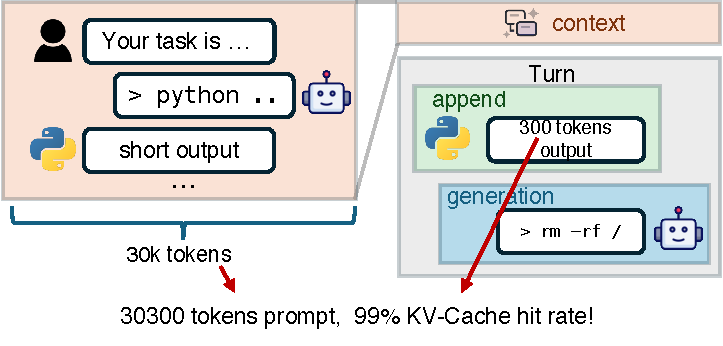
\includegraphics[width=\linewidth]{figures/workload}
  \vspace{-0.3in}
  \caption{\normalfont 智能体轨迹示例。}
  % \vspace{-0.2in}
  \label{fig:workload}
\end{figure}

LLM 越来越多地支撑\emph{智能体}应用：这些应用在长期 session 中进行多轮推理，并与环境交互，例如执行终端命令、运行代码，或请求人类反馈。
如 \autoref{fig:workload} 所示，在典型的\emph{一轮}中，模型接收一个由先前\emph{上下文}和新\emph{追加 token}（通常是工具输出或用户输入）组成的 prompt，并\emph{生成}下一步动作或回复。一次完整智能体运行是一条包含数十轮甚至数百轮的\emph{轨迹}：上下文逐轮增长，最长可达到一百万 token~\cite{claudeopus46, googlegemini3pro}。
由于大部分上下文都会跨轮复用，在我们的 trace 中通常超过 95\% 的 token 会被复用，因此每轮中的绝大多数 token 都能命中 KV-Cache；只有新追加的上下文需要执行 prefill 计算。由于智能体轨迹极长，像 Mooncake~\cite{FAST25:Mooncake} 这类基于 DRAM 和 HBM 的 KV-Cache 存储只能保存很小一部分 KV-Cache，因此必须使用容量更大且成本更低的外部 SSD 型 KV-Cache 存储~\cite{3FS}。

智能体 LLM 推理工作负载也广泛存在于智能体 LLM 训练中，这类训练通常采用\emph{强化学习}（RL）方法。在典型 RL 训练循环中，智能体 LLM 首先进入\emph{rollout} 阶段，被提示生成大量多步智能体轨迹。随后，这些轨迹会由单独的奖励模型打分。最后，LLM 参数被更新，以提高高分输出的概率并降低低分输出的概率。在 rollout 阶段，大量数据（例如奖励模型和优化器状态）会被卸载到主机 DRAM，进一步压缩可用于 KV-Cache 的 DRAM 空间。这进一步强化了对外部高容量 KV-Cache 存储的需求，以便高效容纳长智能体 rollout 上下文。

\subsection{现代 AI 数据中心架构}

现代 AI 数据中心是为大规模生成式 AI 训练和推理工作负载专门构建的逻辑超级计算机。例如，在标准 NVIDIA DGX SuperPOD~\cite{nvidia2023superpod} 中，每个节点配备 8 块 Hopper GPU，并通过高速 NVLink 互联。每块 GPU 都配有一个专用 400 Gbps 计算 NIC（\emph{CNIC}，也称 east-west NIC），用于最大化跨节点通信带宽。独立于计算网络之外，每个节点还配有最高 400 Gbps 的存储 NIC（\emph{SNIC}，也称 south-north NIC），用于快速访问数据集、模型 checkpoint 和磁盘上的 KV cache。

该架构的一个基本原则是计算网络与存储网络彼此隔离~\cite{zhao2025insights}。这种隔离对于同时最大化存储性能和应用性能至关重要。通过将 GPU 之间高强度的 east-west 计算流量与存储流量隔离，该架构可以防止二者互相干扰，并显著降低计算通信延迟。即使在读取大型数据集或写入 TB 级模型 checkpoint 等数据密集型任务期间，该设计也能保证 GPU 间通信保持高度可靠且可预测。
